\documentclass[times, utf8, zavrsni]{fer}
\usepackage{booktabs}

% Linkano kazalo
\usepackage[hidelinks]{hyperref}

\usepackage{color}
\usepackage{listings}
\usepackage{multirow}
\definecolor{javared}{rgb}{0.6,0,0} % for strings
\definecolor{javagreen}{rgb}{0.25,0.5,0.35} % comments
\definecolor{javapurple}{rgb}{0.5,0,0.35} % keywords
\definecolor{javadocblue}{rgb}{0.25,0.35,0.75} % javadoc
\definecolor{javalinenum}{rgb}{0.25,0.25,0.25} % line numbers
\lstset{language=Java,
basicstyle=\ttfamily,
keywordstyle=\color{javapurple}\bfseries,
stringstyle=\color{javared},
commentstyle=\color{javagreen},
morecomment=[s][\color{javadocblue}]{/**}{*/},
numbers=left,
numberstyle=\tiny\color{javalinenum},
stepnumber=1,
numbersep=15pt,
tabsize=4,
showspaces=false,
showstringspaces=false}
\renewcommand{\lstlistingname}{Isječak}

\lstset{
     literate=%
         {ć}{{\'c}}1
         {Ć}{{\'C}}1
         {č}{{\v{c}}}1
         {Č}{{\v{C}}}1
         {ž}{{\v{z}}}1
         {Ž}{{\v{Z}}}1
         {š}{{\v{s}}}1
         {Š}{{\v{S}}}1
}

\newtheorem{relation}{Relacija}[section]
\usepackage{courier}

\usepackage[most]{tcolorbox}
\usepackage{pdfpages}

\newtcolorbox{myframe}[1][]{
  enhanced,
  arc=0pt,
  outer arc=0pt,
  colback=white,
  boxrule=0.8pt,
  #1
}

\begin{document}

% Uključi svu bibliografiju!! -- dodati iza \begin{document}
\nocite{*}

\thesisnumber{4899}

\title{Web aplikacija za upravljanje rasporedom aktivnosti}

\author{Juraj Juričić}

\maketitle

% Ispis stranice s napomenom o umetanju izvornika rada. Uklonite naredbu \izvornik ako želite izbaciti tu stranicu.
%\izvornik

\includepdf[pages={1}]{resources/izvornik.pdf}

% Dodavanje zahvale ili prazne stranice. Ako ne želite dodati zahvalu, naredbu ostavite radi prazne stranice.
\zahvala{}

\tableofcontents

\chapter{Uvod}\label{uvod}
Planiranje i raspoređivanje aktivnosti svakodnevni je problem koji može postati vrlo složen kad govorimo o velikom broju zadataka, a uobičajeno pripada u razred $\mathcal{NP}$-teških problema\footnote{Razred $\mathcal{NP}$-teških problema obuhvaća probleme za koje nema za sada poznato polinomijalnog rješenje.}. Kako aktivnosti u svakodnevnom životu (radu) može biti puno, pojavljuje se potreba za dobrom organizacijom aktivnosti s obzirom na njihovo trajanje, rok te eventualno prioritet.

U okviru ovog rada razmatrat će se i rješavati problem automatiziranog raspoređivanja zadataka u kontekstu osobnog rasporeda. Želimo projektirati i napraviti sustav koji dani ulazni skup zadataka raspoređuje u zadani raspored, pritom poštujući određena ograničenja. Na samom početku možemo pretpostaviti dva ograničenja, uvjeta na problem, kako bismo lakše objasnili generalnu ideju problema i rješenja istog.

\paragraph{Uvjet neistovremenosti} U svakom danom trenutku rasporeda može postojati jedan ili niti jedan događaj; moguće je obavljati najviše jednu aktivnost. Ovaj uvjet zadatka možemo slobodno uvesti temeljem činjenice da slažemo \textit{osobni raspored} -- ako postoji potreba za organizacijom osobnih zadataka, to su često zadaci za koje je potrebno odvojiti vrijeme te se na njih fokusirati, a samim time korisnici ne mogu obavljati više takvih zadatka odjednom (engl. \textit{multitasking}).

\paragraph{Diskretizacija vremena} Nastavno na prethodnu pretpostavku, zadaci koje raspoređujemo u pravilu su duljeg trajanja -- nema smisla u kontekstu osobnog rasporeda planirati obavljanje zadatka koje će trajati nekoliko sekundi, pa čak i samo nekoliko minuta. U okviru rješavanja problema, pretpostavit ćemo da niti jedan zadatak ne traje kraće od jedne minute. U praksi, često će zadaci trajati minimalno 10 minuta, što ćemo imati na umu kod projektiranja određenih dijelova sustava.

\paragraph{}

Na ova dva uvjeta ćemo temeljiti izradu sustava, no mehanizmi slični onima opisanim u ovom radu mogu se generalizirati i na slične probleme. Takvi problemi mogu pak uključivati raspoređivanje aktivnosti među većim brojem osoba (npr. organiziranje poslova među zaposlenicima u poduzeću) ili među različitim skupinama ljudi (npr. odjelima u poduzeću).

Ovaj problem raspoređivanja zadataka može se predstaviti kao višekriterijski optimizacijski proble -- cilj je pronaći onaj raspored koji prema određenim kriterijima najbolje (ili \textit{dovoljno dobro}) zadovoljava ulazne parametre, a da pri tome ne krši zadana ograničenja. Za rješavanje ovog optimizacijskog problema poslužit ćemo se genetskim algoritmom, tako da problem zapravo postaje optimizacija crne kutije (engl. \textit{black-box optimisation)}, a najveći posao tad postaje definiranje reprezentacije rješenja prikladne za upotrebu u genetskom algoritmu\footnote{Kodiranje problema, vidi \ref{kodiranje problema}} te definiranje funkcije (odnosno funkcija) dobrote (engl. \textit{fitness function}) rješenja (odnosno rasporeda).

Na početku, u poglavlju \ref{definicija}, definirat ćemo ulazne parametre sustava i elemente željenog rješenja. Također ćemo definirati način evaluacije rasporeda, odnosno određivanja što čini raspored \textit{dobrim}. U poglavlju \ref{implementacija} ćemo se osvrnuti na neke dijelove arhitekture sustava (korištene biblioteke, modele i evaluacijske funkcije) te njihovu implementaciju u programskom jeziku Java. U poglavlju \ref{primjena genetskog algoritma} bavit ćemo se genetskim algoritmom za rješavanje problema raspoređivanja zadataka te praktičnim svojstvima njegovih dijelova. Pobliže ćemo se upoznati s operatorima selekcije, križanja i mutacije te implementacijom pomoću biblioteke Jenetics koja se koristi kao platforma genetskog algoritma. Na kraju ćemo u poglavlju \ref{web aplikacija} napraviti jednostavno web sučelje za korištenje sustava.% Konačno, u poglavlju \ref{primjeri} proučit ćemo nekoliko primjera korištenja sustava te načine na koji različiti ulazni parametri utječu na dobiveni rezultat.

\chapter{Problem raspoređivanja aktivnosti}\label{definicija}
Prilikom definiranja problema raspoređivanja, korisnik zadaje skup aktivnosti koje sustav treba rasporediti, skup postojećih fiksnih zadataka (odnosno postojeći raspored) te parametre algoritma. Zadatak sustava je složiti \textit{dobar} raspored zadanih aktivnosti, uzimajući u obzir ostale parametre.

\section{Ulazni podaci}\label{ulazni podaci}

\subsection{Aktivnost}
Osnovni entitet ovog problema je \textbf{aktivnost}. Aktivnost predstavlja neku radnju (posao, zadatak) koja mora biti raspoređena u konačno rješenje (raspored). Atributi svake aktivnosti su:
\begin{itemize}
  \item \textbf{naziv},
  \item \textbf{trajanje} - vrijeme (u minutama, satima, ...),
  \item \textbf{rok} (engl. \textit{deadline}) - trenutak u vremenu (konkretan dan i vrijeme),
  \item \textbf{prioritet} (\textit{opcionalno}) - cijeli broj, manja vrijednost predstavlja viši prioritet
\end{itemize}

\paragraph{Rok} Rok predstavlja trenutak u vremenu do kojeg \textit{bi bilo dobro da se aktivnost dovrši}. Rok \textbf{nije tvrdo ograničenje} (engl. \textit{hard constraint})\footnote{Tvrda ograničenja su ona ograničenja koja \textbf{moraju} biti zadovoljena da bi rješenje bilo legalno -- ako rješenje krši neko od tvrdih ograničenja, ne možemo ga smatrati ispravnim.} zbog toga što je moguće zadati ulazne parametre takve da nije moguće složiti raspored u kojem aktivnosti nikad ne prelaze rokove. Ipak, trebamo se pobrinuti da sustav poštuje rokove što je više moguće.

\paragraph{Prioritet} Prioritet određuje kojim redoslijedom se pojedine aktivnosti, uz pretpostavku da niti jedna od njih ne krši rok, trebaju odvijati. Zadan je cjelobrojnom vrijednošću, pri čemu bi se aktivnost s manjom cjelobrojnom vrijednošću prioriteta (višim prioritetom) trebala izvršavati prije aktivnosti s većom cjelobrojnom vrijednošću prioritetom.

\paragraph{}

Nije nužno da se pojedina aktivnost započne i dovrši odjednom; moguće je aktivnosti podijeliti na manje dijelove te ih takve rasporediti u konačan raspored. Štoviše, u pojedinim situacijama\footnote{npr. aktivnosti koje \textit{dugo} traju -- vidi primjer s učenjem za ispit} to će biti i poželjno. Ipak, bitan je uvjet da ukupno trajanje aktivnosti ostane nepromijenjeno.

Za primjer uzmimo dvije aktivnosti - \textbf{pisanje domaće zadaće (2h)} i \textbf{učenje za ispit (18h)}. Pisanje domaće zadaće, kako traje 2h, može se odraditi "u jednom sjedenju". S druge strane, učenje za ispit za koje nam treba 18h, nije nešto što bih preporučio raditi odjednom, stoga tu aktivnost možemo razlomiti na 3 dijela po 6h i rasporediti kroz više dana.

\subsection{Fiksni događaj}\label{fiksni dogadaj}
\textbf{Fiksni događaj} predstavlja unaprijed zadan \textbf{događaj} kojeg sustav ne smije mijenjati te koji mora biti smješten u konačno rješenje (raspored) na točno onom mjestu na kojem je zadan, s točno zadanim trajanjem. Iz ovoga i uvjeta \textit{neistovremenosti} slijedi da se aktivnosti ne mogu rasporediti u vrijeme koje bi se preklapalo s fiksnim događajem.

Atributi fiksnog događaja su:
\begin{itemize}
  \item \textbf{naziv},
  \item \textbf{vrijeme početka} - trenutak u vremenu (konkretan dan i vrijeme),
  \item \textbf{vrijeme kraja} - trenutak u vremenu (konkretan dan i vrijeme)
\end{itemize}

\subsection{Parametri algoritma}
Očito je da postoji \textit{mnogo} različitih rasporeda za dani ulazni skup aktivnosti i fiksnih događaja. Kako bi korisnik mogao odrediti koji od rasporeda aktivnosti njemu više odgovara, sustavu se mogu predati određeni parametri evaluacije rasporeda. O tim će parametrima biti riječi u \ref{evaluacija rasporeda}

\section{Elementi rješenja problema raspoređivanja aktivnosti}\label{elementi rjesenja}
Iz zadanog skupa ulaznih parametara, sustav mora generirati rješenje:
\begin{itemize}
  \item koje zadovoljava uvjete navedene u postavci zadatka (vidi poglavlje \ref{uvod}),
  \item koje sadrži raspoređene sve unesene aktivnosti,
  \item za koje vrijedi da se niti jedna aktivnost vremenski ne \textit{preklapa} s nekim od fiksnih događaja
\end{itemize}

Ispravno (legalno) rješenje je konačan \textbf{raspored} aktivnosti koji sadrži raspoređene sve zadane aktivnosti u punom trajanju te sve zadane fiksne događaje na nepromijenjenim mjestima, a da se niti jedna aktivnost ne preklapa s drugom aktivnošću ili fiksnim događajem.

\paragraph{Događaj} \textbf{Događaj} je osnovni element rasporeda aktivnosti, a može biti \textbf{generiran} iz zadane aktivnosti (prilikom raspoređivanja aktivnosti) ili može biti \textbf{zadan} na ulazu kao fiksni događaj. Događaj je definiran svojim \textbf{početkom} i \textbf{trajanjem}.

\paragraph{Raspored} \textbf{Raspored} predstavlja skup događaja. Zbog uvjeta \textit{neistovremenosti}, u svakom trenutku može se odvijati najviše jedan događaj. Raspored je i konačno rješenje problema raspoređivanja, a može se \textbf{evaluirati}, pri čemu načelno želimo kao konačno rješenje pronaći \textit{najbolje ocijenjen}\footnote{Za ocjenjivanje (evaluaciju) rasporeda služimo se evaluacijskim funkcijama -- vidi \ref{evaluacija rasporeda}.} raspored.

\section{Evaluacija rasporeda}\label{evaluacija rasporeda}
Kako bismo problem raspoređivanja mogli prikazati kao optimizacijski problem, svaki raspored moramo moći evaluirati - dodijeliti mu određenu mjeru dobrote. Očito je da ovdje postoji potreba za definiranjem što su zapravo svojstva \textit{dobrog} rasporeda, stoga ćemo ovdje odrediti neka od pravila. Svako pravilo predstavlja funkciju dobrote kojoj je domena \textit{skup svih rasporeda}, a kodomena \textit{skup realnih brojeva} $\mathbb{R}$. Konačna funkcija evaluacije rasporeda tada se može predstaviti kao linearna kombinacija svih funkcija pravila.

Kako je kriterij što raspored čini \textit{dobrim} subjektivan -- varira od korisnika do korisnika te od jedne situacije za koju se aktivnosti raspoređuju do druge -- pravilima (odnosno funkcijama pravila) ćemo dodijeliti parametre koje korisnik može podešavati. Mijenjanjem parametara pravila može se drastično promijeniti konačni oblik rasporeda za isti ulaznih skup zadataka i ograničenja.% Nekoliko primjera koji to ilustriraju dano je u poglavlju \ref{primjeri}.

U ovom ćemo odjeljku spomenuti moguća pravila koja utječu na evaluaciju, njihove parametre te željeno ponašanje, a u \ref{evaluacijske funkcije} se osvrnuti na implementaciju istih.

\paragraph{Neprekinutost aktivnosti} Svaka aktivnost može biti podijeljena na više dijelova, što u slučajevima dugotrajnih aktivnosti može biti korisno. S druge strane, raspored u kojem su kratke aktivnosti podijeljene na mnogo dijelova vrlo vjerojatno nije dobar raspored. Na primjer, aktivnost od pola sata koja je podijeljena na 15 dijelova po 2 minute, s puno drugih aktivnosti između, nema previše smisla.

Uvedimo parametar $n$: $n \in \left[-1,1\right] \cap \mathbb{R}$. Ako je vrijednost ovog parametra \textbf{pozitivna}, rasporedi koji imaju cjelovitije (manje razlomljene) aktivnosti će biti ocijenjeni kao \textbf{bolji}. Suprotno, ako je vrijednost \textbf{negativna}, boljima će se smatrati oni rasporedi koji imaju više manjih dijelova istih aktivnosti.

Također, htjeli bismo imati mogućnost dodatno kazniti (ili u slučaju negativnog $n$ nagraditi) sekvence aktivnosti koje traju kraće od nekog praga (npr. koje traju manje od 5 minuta i sl.). Uvedimo taj prag kao parametar $t$: $t \in \mathbb{N}$.

\paragraph{Poštivanje roka} Svaka aktivnost ima zadani \textbf{rok} do kojeg mora biti obavljena, no taj rok, kao što je već navedeno u \ref{ulazni podaci}, ne predstavlja \textit{tvrdo ograničenje}. Ipak, očekujemo da je ocjena rasporeda tim \textbf{veća} što \textbf{manje aktivnosti prelazi zadani rok}. Uz to, možemo dodatno povećati ocjenu rasporeda ako je neka od aktivnosti završila prije roka.

Uvedimo dva nova parametra - $r_{kasno}$ i $r_{rano}$: $r_{kasno} \in \left[0,\infty \right>$, $r_{rano} \in \left[0,\infty \right>$. Što je $r_{kasno}$ veći, to će veća biti \textbf{kazna} po trenutku kašnjenja pojedine aktivnosti. Slično, što je $r_{rano}$ veći, to će veća biti \textbf{nagrada} po trenutku ranog završetka pojedine aktivnosti. Uočite da oba parametra mogu biti $0$, što označava da u tom slučaju nema kazne, odnosno nagrade.

\paragraph{Poštivanje prioriteta} Aktivnosti mogu imati zadan i \textbf{prioritet} koji određuje redoslijed kojim bi se aktivnosti trebale odvijati ako ne krše svoj rok. Samim time, ovo pravilo treba imati slabiji utjecaj od prethodnog (poštivanje roka).

Uvedimo parametar $p : p \in \left[0,\infty\right>$ koji linearno određuje veličinu nagrade ili kazne koju raspored dobiva s obzirom na zadovoljavanje uvjeta prioriteta.

\paragraph{Težine funkcija} Svako od ovih pravila možemo individualno podešavati, a konačna evaluacija rješenja dobiva se linearnom kombinacijom rezultata pravila. Konačnu evaluacijsku funkciju možemo formalno zapisati kao u \ref{linearna kombinacija}:
\begin{equation}\label{linearna kombinacija}
f(x) = \sum_{i=1}^{n} w_i f_i(x)
\end{equation}
pri čemu je $x$ raspored koji evaluiramo, $f_i$ pojedina funkcija (pravilo), $w_i$ težina (engl. \textit{weight}) pripadne funkcije, a $n$ broj funkcija (u našem slučaju 3). Vrijedi: $w_i \in \left[0, \infty\right>$.

Iz ovoga je potrebno definirati još 3 ulazna parametra $w_i$ -- težine pojedinih funkcija.

\chapter{Implementacija rješenja problema raspoređivanja aktivnosti}\label{implementacija}

\section{Biblioteke}
Sustav ćemo implementirati u programskom jeziku Java, oslanjajući se na biblioteku \textbf{Jenetics}\footnote{http://jenetics.io} za genetski algoritam. Za web dio aplikacije koristit ćemo \textbf{Spark Framework}\footnote{http://sparkjava.com}.

\paragraph{Jenetics} \textit{Jenetics} je biblioteka otvorenog k{\^o}da koja nudi funkcionalnost genetskog algoritma, s već implementiranom podrškom za česte koncepte genetskog algoritma. Uključuje nekoliko često korištenih operatora selekcije, križanja i mutacije te nudi jednostavno sučelje za implementaciju svojih operatora. Cijelo sučelje biblioteke se temelji na \textbf{Java 8 tokovima}\footnote{Java stream API} te je većina operacija paralelizirana, imajući na umu višedretvenost.

\paragraph{Spark Framework} \textit{Spark Framework} je "micro" radni okvir za izradu web aplikacija manjih opsega napisan u Javi. Omogućuje vrlo brzu izradu jednostavnijih web aplikacija s naglaskom na performansama i minimalizmu pisanja. Kako je kod ove aplikacije fokus na algoritamskom dijelu, web dio je minimalan što ga čini odličnim izborom.

\section{Modeli}
\paragraph{Task} Nepromjenjivi (engl. \textit{immutable}) model \texttt{Task} predstavlja pojedinu aktivnost. Prisjetimo se, svaka aktivnost je definirana \textbf{nazivom}, \textbf{trajanjem}, \textbf{rokom} te \textbf{prioritetom}, što su ujedno i atributi ovog modela -- prikazano u isječku \ref{code:task}:
\begin{lstlisting}[language=java, caption=Razred Task, label={code:task}]
public class Task {
	public final String name;
	public final Duration duration;
	public final LocalDateTime deadline;
	public final LocalDateTime earliest;
}
\end{lstlisting}

\paragraph{Calendar} Model \texttt{Calendar} predstavlja konačnu instancu rasporeda, a određen je skupom svih događaja\footnote{CalendarEvent} koji se nalaze u njemu. Sam podatkovni model je vrlo jednostavan (jedan atribut -- skup \texttt{eventSet}), no mora nuditi i metode za rad s događajima u kalendaru. Isječak \ref{code:calendar} sadrži pojednostavljeno sučelje razreda \textbf{\texttt{Calendar}}, bez implementacije:
\begin{lstlisting}[language=java, caption=Razred Calendar, label={code:calendar}]
public class Calendar implements Iterable<CalendarEvent> {
	private NavigableSet<CalendarEvent> eventSet;
	
	public boolean add(CalendarEvent event)
	public void addAll(Calendar other)
	public NavigableSet<CalendarEvent> getEventSet()
	
	public Calendar from(LocalDateTime from,
		boolean inclusive)
	public Calendar to(LocalDateTime to, boolean inclusive)
	public Calendar fromTo(LocalDateTime from,
		LocalDateTime to, boolean inclusive)
		
	public int size()
}
\end{lstlisting}
Za prikaz kalendara u web aplikaciji koriste se metode \texttt{from}, \texttt{to} te \texttt{fromTo}, koje vraćaju živi pogled (engl \textit{live view)} na traženi isječak kalendara.

\paragraph{CalendarEvent} Model \texttt{CalendarEvent} predstavlja jedan zapis događaja u kalendaru. Pojedini događaj može biti ili \textbf{generiran} temeljem neke od raspoređenih aktivnosti (pri čemu događaj može biti i samo dio aktivnosti) ili neki fiksni događaj (u tom slučaju je smješten temeljem korisničkog unosa i predstavlja cijeli fiksni događaj).

S obzirom na potrebe kalendara, događaj je definiran svojim \textbf{nazivom}, \textbf{trenutkom početka}, \textbf{trenutkom završetka} (ili \textbf{trajanjem}). Ipak, poželjno je da pamtimo i kako je pojedini događaj nastao, stoga dodajmo još jedan atribut - \textbf{tip}. Isječak \ref{code:calendarEvent} prikazuje osnovne atribute razreda \texttt{CalendarEvent}.
\begin{lstlisting}[float, language=java, caption=Razred CalendarEvent, label={code:calendarEvent}]
public class CalendarEvent implements Comparable<CalendarEvent> {
    private String title;
    private final LocalDateTime eventStart;
    private final LocalDateTime eventEnd;
    private final Duration duration;
    private EventType eventType;
}
\end{lstlisting}

Prilikom stvaranja objekta tipa \texttt{CalendarEvent}, automatski se računa trajanje i sprema u člansku varijablu \texttt{duration}, radi bržeg naknadnog dohvata.

\section{Diskretizacija vremena}\label{diskretizacija vremena}
Iako je vrijeme kontinuirana veličina, mi ćemo ga promatrati kroz diskretne vrijednosti. Uvedemo pojam \textit{trenutka}, koji predstavlja određeni fiksni period (npr. 1 minutu) -- u tom slučaju će se 1 sat sastojati od 60 trenutaka. To trajanje jednog trenutka dan je na ulazu sustava, a praktično je za tu primjenu iskoristiti neku vrijednost koja dijeli 60 minuta (npr. 10 minuta, 20 minuta, 30 minuta). Ono predstavlja vremensku preciznost sustava.

Raspored tako postaje kao niz \textit{trenutaka}, od kojih svaki može (ali i ne mora) imati dodijeljenu aktivnost (i to najviše jednu, prema uvjetu neistovremenosti). Implementacijski, potrebno je pamtiti koliko je trajanje jednog trenutka te uvesti razrede koji će predstavljati trenutke. Uvedimo apstraktni razred \texttt{Moment} te konkretne razrede \texttt{EmptyMoment}, \texttt{TaskMoment} i \texttt{FixedMoment}.

\paragraph{Moment} Osnovni nadrazred \texttt{Moment} sadrži referencu na \textit{tvornicu} sekvenci koja ga je stvorila -- objekt tipa \texttt{MomentSeqFactory} -- a koja sadrži podatak o trajanju jednog trenutka. Uz to, nudi metodu \texttt{similar(Moment)} za usporedbu dva objekta tipa \texttt{Moment}.  Razredi koji nasljeđuju \texttt{Moment} trebaju biti nepromjenjivi (engl. \textit{immutable}). Isječak k\^{o}da ovog razreda prikazan je u isječku \ref{code:moment}:

\begin{lstlisting}[language=java, caption=Apstraktni razred Moment, label={code:moment}]
public abstract class Moment {
    public final MomentSeqFactory creator;

    protected Moment(MomentSeqFactory creator) {
        this.creator = creator;
    }

    public abstract String toString();
    public abstract boolean similar(Moment o);
    
    // ...
}
\end{lstlisting}

\paragraph{EmptyMoment} Razred \texttt{EmptyMoment} predstavlja trenutak bez događaja te ne pruža sučelje različito od nadrazreda \texttt{Moment}. Metoda \texttt{similar(Moment)} vraća vrijednost \texttt{true} ako i samo ako je objekt s kojim se vrši usporedba također tipa \texttt{EmptyMoment}.

\paragraph{TaskMoment} Trenutci koji sadrže pojedine dijelove aktivnosti predstavljeni su razredom \texttt{TaskMoment}. Ovaj razred, uz sučelje nadrazreda \texttt{Moment}, dodatno nudi podatak o aktivnosti koju predstavlja te redni broj trenutka za danu aktivnost. Pojednostavljeni k\^{o}d razreda \texttt{TaskMoment} dan je u isječku \ref{code:taskMoment}:

\begin{lstlisting}[language=java, caption=Razred TaskMoment, label={code:taskMoment}]
public class TaskMoment extends Moment {
	public final Task task;
	public final int partNumber;
	
	public boolean similar(Moment o) {
        if (o == null) return false;
        if (!(o instanceof TaskMoment)) return false;

        return this.task.equals(((TaskMoment) o).task);
    }
    
    public boolean equals(Object o) {
        if (this == o) return true;
        if (!(o instanceof TaskMoment)) return false;
        if (!super.equals(o)) return false;

        TaskMoment that = (TaskMoment) o;

        if (partNumber != that.partNumber) return false;
        return task.equals(that.task);
    }
}
\end{lstlisting}
Primijetimo razliku između metoda \texttt{similar(Moment)} i \texttt{equals(Object)}: metoda \texttt{similar} će vratiti vrijednost \texttt{true} ako je aktivnost koju ovaj trenutak predstavlja jednaka aktivnosti trenutka s kojim vršimo usporedbu, čak i ako im redni broj nije jednak, dok metoda \texttt{equals} ima dodatan uvjet provjere na redni broj trenutka u aktivnosti.

\paragraph{FixedMoment} Trenutci koji sadrže dijelove fiksnih događaja predstavljeni su razredom \texttt{FixedMoment}. Slično kao i \texttt{TaskMoment}, ovaj razred sadrži referencu na fiksni događaj koji predstavlja te redni broj trenutka za dani fiksni događaj. Pojednostavljeni k\^{o}d razreda \texttt{FixedMoment} dan je u isječku \ref{code:fixedMoment}:

\begin{lstlisting}[language=java, caption=Razred FixedMoment, label={code:fixedMoment}]
public class FixedMoment extends Moment {
	public final int partNumber;
    public final CalendarEvent event;
	
	public boolean similar(Moment o) {
        if (o == null) return false;
        if (!(o instanceof FixedMoment)) return false;

        return this.event.equals(((FixedMoment) o).event);
    }
}
\end{lstlisting}

\section{Evaluacijske funkcije}\label{evaluacijske funkcije}
Kako bismo problem raspoređivanja oblikovali u optimizacijski problem te ga mogli rješavati genetskim algoritmom, potrebno je definirati funkciju dobrote (engl. \textit{fitness function}) rasporeda. U \ref{evaluacija rasporeda} smo naveli 3 funkcije (pravila) koje evaluiraju raspored. Kao što je ondje već navedeno, konačnu evaluacijsku funkciju oblikovat ćemo kao linearnu kombinaciju tih funkcija:
\begin{equation}
f(x) = \sum_{i=1}^{n} w_i f_i(x)
\end{equation}
pri čemu je $x$ raspored koji evaluiramo, $f_i$ pojedina funkcija, $w_i$ težina (engl. \textit{weight}) pripadne funkcije, a $n$ broj funkcija (u našem slučaju 3).

Kako se svaka od funkcija pokreće jednom nad svakom jedinkom populacije, a genetski algoritam radi s velikim populacijama i velikim brojem generacija, evaluacijska funkcija često postaje usko grlo (engl. \textit{bottleneck}) performansi, stoga je bitno obratiti pažnju i na složenost individualnih evaluacijskih funkcija.

\subsection{Neprekinutost aktivnosti}\label{fja:neprekinutost aktivnosti}
Kao što je navedeno u poglavlju \ref{evaluacija rasporeda}, ova funkcija je definirana parametrom $n$, a želimo postići da, u slučaju pozitivnog $n$, funkcija raste s duljim trajanjem pojedine aktivnosti, a za negativni $n$ vrijedi obrat (funkcija pada).

Glavni zadatak koji ova funkcija mora ponuditi je praćenje duljine sekvence iste aktivnosti, počevši na početku rasporeda. Jednom kad se aktivnost promijeni, sekvenca prestaje.
Razmotrimo algoritam u isječku \ref{code:duljina sekvence}:

\begin{lstlisting}[language=java, caption=Algoritam određivanja duljine sekvence aktivnosti, label={code:duljina sekvence}]
// Moments[] moments ...

double score = 0;
int sequenceLength = 1;
Moment previous = moments[0];

for (int i = 1; i < moments.length; i++) {
	Moment current = moments[i];
	if (current.similar(previous)) {
		sequenceLength++;
	} else {
		score += evaluate(previous, sequenceLength);
		sequenceLength = 1;
		previous = current;
	}
}

return score;
\end{lstlisting}
Složenost ovog algoritma je $\mathcal{O}(n)$ gdje $n$ predstavlja broj trenutaka, a algoritam se koristi u metodi \texttt{apply()} razreda \texttt{TasksSequenceFunction}. Preostaje nam napisati metodu \texttt{evaluate(Moment, int)} (s linije 12), koja ovisno o duljini sekvence računa \texttt{double} ocjenu sekvence (parametrizirano prema $n$).

Parametar $n$ određuje koliko brzo ova funkcija treba rasti s obzirom na duljinu sekvence.  Istovremeno, želimo da funkcija ima eksponencijalni rast, odnosno da dulje sekvence imaju eksponencijalno veću ocjenu. Imajući na umu domenu parametra $n \in \left[-1, 1\right]$, definirajmo funkciju \ref{fja:sgnduljina}:

\begin{equation}\label{fja:sgnduljina}
f(duljina) = sgn(n) \cdot duljina^{|{n}\cdot{\psi}|}
\end{equation}
pri čemu je $duljina$ duljina sekvence, $n$ parametar funkcije, a $\psi$ faktor skaliranja, koji služi kako bi se domena parametra $n$ skalirala na veći raspon. Generalna ideja iza (\ref{fja:sgnduljina}) je da se parametar $n$ skalira kako bi konačna vrijednost bila istog reda veličine kao i ostale evaluacijske funkcije, a da eksponent pritom uvijek bude pozitivan broj. Ako je $n$ negativan, to će se odraziti u konačnom predznaku rezultata.

Parametar $t$ određuje prag ispod kojeg se mijenja ponašanje funkcije - za pozitivan $n$ se sekvence kraće od $t$ kažnjavaju, umjesto da se nagrađuju.

\begin{lstlisting}[language=java, caption=Ocjena duljine sekvence]
double evaluate(Moment previous, int sequenceLength) {
	// this.param_t - ulazni parametar t
	// this.param_n - ulazni parametar n
	double sgn = Math.signum(this.param_n);
	if (sequenceLength < this.param_t) {
		sgn *= -1;
	}

	return sgn *
		Math.pow(sequenceLength,
			Math.abs(this.param_n * this.scaleFactor)
		);
}
\end{lstlisting}
Linije 5-7 se brinu za inverzno ponašanje kod kratkih aktivnosti - ako je duljina sekvence kraća od $t$, predznak parametra $n$ će biti promijenjen za ovu iteraciju.

\subsection{Poštivanje roka}\label{fja:postivanje roka}
Prisjetimo se poglavlja \ref{evaluacija rasporeda} -- svaka aktivnost može imati rok (koji predstavlja \textit{meko ograničenje}) do kojeg bi trebala biti obavljena. Zadatak ove evaluacijske funkcije je kazniti rasporede u kojima aktivnosti nisu odrađene u roku te eventualno nagraditi rasporede u kojima se aktivnosti obavljaju prije roka. Ova funkcija je definirana parametrima $r_{kasno}$ i $r_{rano}$.

Implementacija ove funkcije je jednostavna, a temelji se -- kao i prethodna funkcija -- na slijednoj iteraciji po svim trenucima rješenja. Za svaki trenutak računamo koliko je aktivnost koju taj trenutak predstavlja udaljena od svojeg roka (u pozitivnom ili negativnom smjeru) te rasporedu dodajemo ili oduzimamo vrijednost u skladu s parametrima $r_{kasno}$ i $r_{rano}$. Razmotrimo algoritam u isječku \ref{code:deadline}:

\begin{lstlisting}[language=java, caption=Algoritam određivanja kašnjenja trenutaka, label={code:deadline}]
// Moments[] moments ...

double score = 0;
for (int i = 0; i < moments.length; i++) {
    if (!(moments[i] instanceof TaskMoment)) continue;

    LocalDateTime time = mapTimePoint(i);

    Duration late = Duration.between(
    	moments[i].task.deadline, point
    );
    score += evaluate(late);
}

return score;
\end{lstlisting}
Metoda \texttt{mapTimePoint(int)} za danu poziciju gena u kromosomu (počevši od 0) vraća trenutak u vremenu koji taj gen predstavlja, i to uzimajući u obzir fiksne događaje\footnote{Kao što ćemo vidjeti u \ref{fiksni dogadaji}, fiksni događaji se ne zapisuju u sam kromosom već čuvaju u posebnoj listi. Metoda \texttt{mapTimePoint(int)} uzima u obzir tu listu.}. Preostaje nam definirati matematičku funkciju kojom određujemo količinu nagrade ili kazne ovisno o količini kašnjenja -- funkcija \texttt{evaluate(Duration)} u prethodnom isječku. Složenost ovog algoritma je $\mathcal{O}(n)$.

Slično kao i kod duljina sekvenci u \ref{fja:neprekinutost aktivnosti}, želimo da za veće kašnjenje raspored bude više kažnjen te ćemo se za to također poslužiti eksponencijalnom funkcijom. Imajući na umu parametre funkcije $r_{kasno}$ i $r_{rano}$, definirajmo funkciju \ref{fja:expdeadline}:

\begin{equation}\label{fja:expdeadline}
f(x)= 
\begin{cases}
    -x^{r_{kasno}}, & \text{za } x\geq 0\\
    x^{r_{rano}},  & \text{inače}
\end{cases}
\end{equation}
pri čemu je $x$ \textbf{kašnjenje} danog trenutka u minutama -- varijabla \texttt{late} s linije 9 u isječku \ref{code:deadline}. Vrijednost $x$-a može biti i negativna, što označava da je trenutak aktivnosti smješten prije roka aktivnosti. Implementacija funkcije \texttt{evaluate(Duration)} je dana u isječku \ref{code:evaluate late}

\begin{lstlisting}[language=java, caption=Ocjena kašnjenja trenutka, label={code:evaluate late}, mathescape]
double evaluate(Duration late) {
	if (late >= 0) {
		return -Math.pow(late, this.rLate);
	} else {
		return Math.pow(late, this.rEarly);
	}
}
\end{lstlisting}

\subsection{Poštivanje prioriteta}\label{fja:postivanje prioriteta}
Prioritet određuje redoslijed kojim se aktivnosti trebaju obavljati, odnosno kojim redoslijedom trebaju biti smještene u raspored. Kako svaka aktivnost može biti podijeljena na više dijelova, javlja se problem odlučivanja koji trenutak odabrati da predstavlja cjelokupnu aktivnost. 

Dogovorno za ovu primjenu biramo \textbf{posljednji} trenutak aktivnosti, budući da upravo taj trenutak određuje kada je aktivnost \textbf{dovršena}. Sada se zadatak ove funkcije može podijeliti u dva dijela:
\begin{enumerate}
  \item određivanje posljednjeg trenutka svake od aktivnosti
  \item provjera redoslijeda aktivnosti s obzirom na prioritet
\end{enumerate}

Prvi korak je trivijalan te se jednostavno može napisati algoritam koji ga izvodi u $\mathcal{O}(n\log{}n)$, a rezultate pohranjuje u sortiranu mapu\footnote{razred \texttt{SortedMap} implementacije \texttt{TreeMap} u programskom jeziku Java} -- vidi isječak \ref{code:deadline_occurence}:

\begin{lstlisting}[language=java, caption=Određivanje posljednjeg trenutka aktivnosti, label={code:deadline_occurence}, mathescape]
SortedMap<Task, Integer> lastOccurence =
    new TreeMap<>((a, b) -> {
        if (a.equals(b)) return 0;
        
        return (a.priority.getAsInt() >=
            b.priority.getAsInt()) ? 1 : -1;
    });

for (int i = 0; i < moments.length; i++) {
    if (!moments[i] instanceof TaskMoment) continue;
    
    lastOccurence.put(moments[i].task, i);
}
\end{lstlisting}
Ključevi mape su aktivnosti, a vrijednosti su indeksi na kojima se nalazi posljednji trenutak pojedine aktivnosti. Lambda izraz koji predajemo konstruktoru \texttt{TreeMap}-a je komparator koji uspoređuje prioritete dviju aktivnosti, no u slučaju da su prioriteti jednaki, također vrati \textbf{1}, kako bi se u mapu mogle pohraniti aktivnosti s jednakim prioritetima.

Jednom kad imamo stvorenu sortiranu mapu \texttt{lastOccurence}, drugi korak funkcije treba proći po svim elementima stvorene mape te provjeriti redoslijed posljednjih elemenata -- u idealnom slučaju, vrijednosti mape (indeksi pojavljivanja) će biti uzlazno sortirani. Funkcija treba nagraditi slučajeve susjednih indeksa kod kojih je drugi veći od prvog, a kazniti suprotne slučajeve. K\^{o}d te funkcije je prikazan u isječku \ref{code:deadline_pt2}:

\begin{lstlisting}[language=java, caption=Provjera redoslijeda aktivnosti, label={code:deadline_pt2}, mathescape]
int size = lastOccurence.size();
int previousPriority = Integer.MIN_VALUE;
int previousIndex = Integer.MAX_VALUE;
double score = 0;
for(Entry<Task, Integer> entry : lastOccurence.entrySet()) {
    if (entry.getKey().priority.orElse(Integer.MIN_VALUE)
        == previousPriority) continue;
        
    if (entry.getValue() > previousIndex) {
        score += parameter * size;
    } else {
        score -= parameter * size;
    }
    
    previousPriority = entry.getKey().priority
        .orElse(Integer.MIN_VALUE);
}
\end{lstlisting}

\chapter{Primjena genetskog algoritma na rješavanje problema raspoređivanja aktivnosti}\label{primjena genetskog algoritma}
\section{Genetski algoritam}\label{genetski algoritam}
Genetski algoritmi su porodica metaheuristika koja svoje ideje temelji na evolucijskom procesu prirodne selekcije. Osnovna ideja iza općeg genetskog algoritma je evoluirati populaciju potencijalnih rješenja primjenom operatora selekcije, križanja i mutacije inspiriranih genetičkom varijacijom i prirodnom selekcijom \citep{mitchell1998introduction}.

Generalna ideja genetskog algoritma je sljedeća: algoritam radi s \textit{populacijom} jedinki, pri čemu je svaka jedinka jedno moguće rješenje zadanog problema. Svaka jedinka sastoji se od najčešće jednog, no moguće i više \textit{kromosoma}. Svaki kromosom se sastoji od niza \textit{gena}. Svaku jedinku možemo \textit{evaluirati}, odnosno odrediti njezinu \textit{dobrotu} (engl. \textit{fitness}). Na početku algoritam stvori početnu populaciju nasumičnih jedinki. Operatorom \textit{selekcije} (engl. \textit{selection}) iz populacije se biraju jedinke koje će postati roditelji. Roditelji pomoću operatora \textit{križanja} (engl. \textit{crossover}) stvaraju djecu, čime se emulira izmjena genetskog materijala (engl. \textit{recombination}). Nad djecom potom djeluje operator \textit{mutacije} (engl. \textit{mutation}). Konačno, operatorom \textit{zamjene} (engl. \textit{reinsertion}) djeca ulaze u populaciju rješenja, čime se zatvara ciklus rada algoritma \citep{book:cupic_optjava}. Taj se ciklus ponavlja više puta, a svaka iteracija algoritma se naziva \textit{generacijom}.

Biblioteka Jenetics koristi varijaciju genetskog algoritma čini je pseudok{\^o}d prikazan u isječku \ref{code:simplepseudoGA}:

\begin{lstlisting}[language=java, caption=Genetski algoritam, label={code:simplepseudoGA}, mathescape]
$g \leftarrow 0$
$P_0 \leftarrow P_{pocetno}$
$F(P_0)$
while !kraj do:
	$g \leftarrow g + 1$
	$S_g \leftarrow select_S(P_{g-1})$
	$O_g \leftarrow select_O(P_{g-1})$
	$O_g \leftarrow alter(O_g)$
	$P_g \leftarrow filter[g_i \geq g_{max}](S_g) + filter[g_i \geq g_{max}](O_g)$
	$F(P_g)$
\end{lstlisting}

Linija (1) postavlja brojač generacija na 0. Linija (2) stvara početnu populaciju, a linija (3) evaluira sve jedinke populacije. Početna populacija $P_{pocetno}$ je implicitno stvorena prije prvog koraka evolucije. Linija (4) povećava brojač generacija. Linije (5) i (6) odabiru populaciju preživjelih jedinki te populaciju novih jedinki (potomaka). Veličine ovih populacija su uvijek u zadanom omjeru \textit{offspringFraction}. Odabrani potomci se križaju i mutiraju u liniji (8). Iduća linija kombinira populacije $S_g$ i $O_g$ -- nakon uklanjanja \textit{mrtvih} jedinki -- u novu populaciju $P_g$. Nove jedinke u populaciji se konačno evaluiraju u liniji (10) \citep{jenetics_userguide}. Ovakva varijanta generacijskog genetskog algoritam uvijek zadržava $1-offspringFraction$ stare populacije, a uvodi $offspringFraction$ novih jedinki.

Proučimo linije (6-8). Operatori selekcije $select_S()$ i $select_O()$ odabiru zadani broj jedinki iz originalne (prethodne) populacije $P_{g-1}$. Nakon linije (7) vrijedi $S_g \subset P_{g-1}$ te je nad tim skupom tek potrebno vršiti odabir roditelja, križanje te mutaciju djece. Za to je zadužena operacija $alter(O_g)$ na liniji(8), čiji je pojednostavljeni pseudok{\^o}d prikazan u isječku \ref{code:alter}:

\begin{lstlisting}[language=java, caption=Operacija alter($O_g$), label={code:alter}, mathescape]
// križanje
$(R_1, R_2) \leftarrow random\_elements(O_g, 2)$
$(D_1, D_2) \leftarrow crossover(R_1, R_2)$

// mutacija
$D_1 \leftarrow mutate(D_1)$
$D_2 \leftarrow mutate(D_2)$

$O_g \leftarrow O_g \setminus \{R_1, R_2\}$
$O_g \leftarrow O_g \cup \{D_1, D_2\}$
\end{lstlisting}

Prvi korak operacije $alter()$ je na liniji (2) -- odabir dva nasumična roditelja iz $O_g$, pri čemu sve jedinke imaju jednaku vjerojatnost da budu odabrane. Na liniji (3) se provodi križanje roditelja operatorom križanja, iz čega nastaju dva potomka $D_1$ i $D_2$. Na linijama (6) i (7) se provodi mutacija svakog od potomaka operatorom mutacije. Konačno, djeca zamjenjuju roditelje u $O_g$. Uočite kako djeca već u idućem koraku mogu postati roditelji.

\section{Kodiranje problema}\label{kodiranje problema}
Dvije osnovne komponente svakog problema koji se rješava genetskim algoritmom su \textit{kodiranje problema} (engl. \textit{problem encoding}) i \textit{evaluacijska funkcija} \citep{whitley1994genetic}. O evaluacijskoj funkciji\footnote{Kada govorimo o evaluacijskoj funkciji, možemo govoriti o funkciji dobrote (engl. \textit{fitness function}) ili funkciji kazne (engl. \textit{cost function}) (engl. \textit{evaluation function}). Cilj genetskog algoritma je maksimizirati funkciju dobrote, odnosno minimizirati funkciju kazne.} kao linearnoj kombinaciji više funkcija dobrote smo govorili u poglavlju \ref{evaluacijske funkcije}. U nastavku ćemo definirati reprezentaciju rješenja kromosomom.

\subsection{Kromosom}\label{kromosom}
Kao što je već rečeno, jedinka predstavlja jedno rješenje zadanog problema, što je u našem slučaju jedan raspored zadataka. Postavlja se pitanje kako najbolje predstaviti raspored zadataka, a da nad njime možemo vršiti operacije križanja i mutacije -- kako treba izgledati kromosom našeg problema?

Kao što je razloženo u poglavlju \ref{diskretizacija vremena}, raspored se sastoji od niza \textit{trenutaka}. Kako je u našem problemu jedinka upravo \textbf{raspored}, ovo možemo iskoristiti kako bismo oblikovali kromosom. Jedinka će imati jedan kromosom kod kojeg svaki gen predstavlja aktivnost koja se "nalazi" u pojedinom trenutku. Prikažemo li raspored na ovaj način, automatski smo zadovoljili uvjet neistovremenosti.

Promotrimo jedan jednostavan slučaj: potrebno je rasporediti dvije aktivnosti -- \textbf{A} i \textbf{B} -- u periodu od 08:00 do 08:15. \textbf{Aktivnost A} traje 5 minuta, a \textbf{aktivnost B} 4 minute. Podijelimo li zadani period na trenutke po 1 minutu, imat ćemo ukupno 15 trenutaka, a aktivnosti \textbf{A} i \textbf{B} traju redom 5, odnosno 4 trenutaka.

\begin{table}[!htbp]
\centering
\caption{Primjer raspoređivanja aktivnosti A i B}
\label{chromosomes-1}
\begin{tabular}{lllllcllllclllllcll}
\multicolumn{3}{c}{08:00} &  &  & \multicolumn{4}{c}{08:05} &  & \multicolumn{4}{c}{08:10} &  &  & \multicolumn{3}{c}{08:15} \\
 & \multicolumn{1}{l|}{} &  &  &  & \multicolumn{1}{l}{} & \multicolumn{1}{l|}{} &  &  &  & \multicolumn{1}{l}{} & \multicolumn{1}{l|}{} &  &  &  &  & \multicolumn{1}{l|}{} &  &  \\ \cline{3-17}
 & \multicolumn{1}{l|}{} & \multicolumn{1}{c|}{A} & \multicolumn{1}{c|}{A} & \multicolumn{1}{c|}{A} & \multicolumn{1}{c|}{A} & \multicolumn{1}{c|}{A} & \multicolumn{1}{c|}{0} & \multicolumn{1}{c|}{0} & \multicolumn{1}{c|}{0} & \multicolumn{1}{c|}{0} & \multicolumn{1}{c|}{0} & \multicolumn{1}{c|}{0} & \multicolumn{1}{c|}{B} & \multicolumn{1}{c|}{B} & \multicolumn{1}{c|}{B} & \multicolumn{1}{c|}{B} &  &  \\ \cline{3-17}
 &  &  &  &  & \multicolumn{1}{l}{} &  &  &  &  & \multicolumn{1}{l}{} &  &  &  &  &  & \multicolumn{1}{l}{} &  &  \\ \cline{3-17}
 & \multicolumn{1}{l|}{} & \multicolumn{1}{c|}{B} & \multicolumn{1}{c|}{B} & \multicolumn{1}{c|}{B} & \multicolumn{1}{c|}{B} & \multicolumn{1}{c|}{0} & \multicolumn{1}{c|}{0} & \multicolumn{1}{c|}{A} & \multicolumn{1}{c|}{A} & \multicolumn{1}{c|}{A} & \multicolumn{1}{c|}{A} & \multicolumn{1}{c|}{A} & \multicolumn{1}{c|}{0} & \multicolumn{1}{c|}{0} & \multicolumn{1}{c|}{0} & \multicolumn{1}{c|}{0} &  &  \\ \cline{3-17}
\end{tabular}
\end{table}

Tablica \ref{chromosomes-1} prikazuje dva kromosoma različitih jedinki -- rasporeda -- za zadani primjer. U prvom (gornjem) slučaju, \textbf{aktivnost A} je raspoređena od 08:00 do 08:05, a \textbf{aktivnost B} od 08:11 do 08:15. U periodu od 08:05 do 08:11 nema aktivnosti, što je označeno nizom nula ($0$). U drugom (donjem) slučaju, \textbf{aktivnost B} je raspoređena od 08:00 do 08:04, a \textbf{aktivnost A} od 08:06 do 08:11. Uočimo kako obje jedinke sadrže iste aktivnosti, ali na različitim mjestima -- geni su \textbf{permutirani}.

Općenito, za zadanu istu instancu problema\footnote{Isti ulazni skup zadataka,  fiksnih događaja i ograničenja}, svako rješenje očigledno mora sadržavati isti skup aktivnosti -- kromosomi rješenja za isti problem se razlikuju samo po permutaciji gena, pa takve kromosome i nazivamo \textbf{permutacijama} ili \textbf{permutacijskim kromosomima}.

\subsection{Fiksni događaji}\label{fiksni dogadaji}
Ostaje pitanje kako u ovaj koncept kromosoma uklopiti fiksne događaje. (Pogrešna) ideja koja se prirodno nameće je fiksne događaje podijeliti na isti način na koji dijelimo aktivnosti te ih smjestiti u kromosom, što je prikazano u tablici \ref{chromosome-fiksni-1} -- aktivnosti \textbf{A} i \textbf{B} su istih parametara kao i u prethodnom primjeru, uz dodani fiksni događaj od 08:05 do 08:10 (označeno slovom \textbf{F}):

\begin{table}[!htbp]
\centering
\caption{Kromosom s fiksnim događajem}
\label{chromosome-fiksni-1}
\begin{tabular}{lllllcllllclllllcll}
\multicolumn{3}{c}{08:00} &  &  & \multicolumn{4}{c}{08:05} &  & \multicolumn{4}{c}{08:10} &  &  & \multicolumn{3}{c}{08:15} \\
 & \multicolumn{1}{l|}{} &  &  &  & \multicolumn{1}{l}{} & \multicolumn{1}{l|}{} &  &  &  & \multicolumn{1}{l}{} & \multicolumn{1}{l|}{} &  &  &  &  & \multicolumn{1}{l|}{} &  &  \\ \cline{3-17}
 & \multicolumn{1}{l|}{} & \multicolumn{1}{c|}{A} & \multicolumn{1}{c|}{A} & \multicolumn{1}{c|}{A} & \multicolumn{1}{c|}{A} & \multicolumn{1}{c|}{A} & \multicolumn{1}{c|}{\textbf{F}} & \multicolumn{1}{c|}{\textbf{F}} & \multicolumn{1}{c|}{\textbf{F}} & \multicolumn{1}{c|}{\textbf{F}} & \multicolumn{1}{c|}{\textbf{F}} & \multicolumn{1}{c|}{0} & \multicolumn{1}{c|}{B} & \multicolumn{1}{c|}{B} & \multicolumn{1}{c|}{B} & \multicolumn{1}{c|}{B} &  &  \\ \cline{3-17}
\end{tabular}
\end{table}

No prema \ref{elementi rjesenja}, fiksni događaji, zadani na ulazu, ne smiju se mijenjati (premještati), a aktivnosti koje raspoređujemo ne smiju se preklapati sa zadanim fiksnim događajima. S druge strane, ideja reprezentacije permutacijskim kromosomom se temelji na tome da se geni u kromosomu smiju slobodno permutirati te da je rješenje legalno \textit{ako je njegov kromosom permutacija kromosoma drugog legalnog rješenja}. U tablici \ref{chromosome-fiksni-2} prikazan je kromosom koji je permutacija onog iz tablice \ref{chromosome-fiksni-1}, ali \textbf{nije legalan} -- fiksni događaj se odvija u pogrešno vrijeme (od 08:01 do 08:06).

\begin{table}[!htbp]
\centering
\caption{Nelegalan kromosom s fiksnim događajem}
\label{chromosome-fiksni-2}
\begin{tabular}{lllllcllllclllllcll}
\multicolumn{3}{c}{08:00} &  &  & \multicolumn{4}{c}{08:05} &  & \multicolumn{4}{c}{08:10} &  &  & \multicolumn{3}{c}{08:15} \\
 & \multicolumn{1}{l|}{} &  &  &  & \multicolumn{1}{l}{} & \multicolumn{1}{l|}{} &  &  &  & \multicolumn{1}{l}{} & \multicolumn{1}{l|}{} &  &  &  &  & \multicolumn{1}{l|}{} &  &  \\ \cline{3-17}
 & \multicolumn{1}{l|}{} & \multicolumn{1}{c|}{0} & \multicolumn{1}{c|}{\textbf{F}} & \multicolumn{1}{c|}{\textbf{F}} & \multicolumn{1}{c|}{\textbf{F}} & \multicolumn{1}{c|}{\textbf{F}} & \multicolumn{1}{c|}{\textbf{F}} & \multicolumn{1}{c|}{A} & \multicolumn{1}{c|}{A} & \multicolumn{1}{c|}{A} & \multicolumn{1}{c|}{A} & \multicolumn{1}{c|}{A} & \multicolumn{1}{c|}{B} & \multicolumn{1}{c|}{B} & \multicolumn{1}{c|}{B} & \multicolumn{1}{c|}{B} &  &  \\ \cline{3-17}
\end{tabular}
\end{table}

Zbog ovoga je potrebno fiksne događaje na drugi način ukomponirati u rješenje. Prema uvjetu zadatka (a i njihovoj definiciji iz \ref{fiksni dogadaj}), fiksni događaji imaju fiksno definirano vrijeme početka i kraja, stoga ih nije dobro smjestiti u kromosom kao gene. Druga ideja koja se nameće je čuvati listu fiksnih događaja neovisno o kromosomu te konačni raspored generirati temeljem kromosoma i liste fiksnih događaja. Kako kromosom tad nema informaciju o fiksnim događajima (a oni ipak utječu na evaluaciju rješenja), evaluacijskim funkcijama se implicitno prosljeđuje\footnote{Listu fiksnih događaja prosljeđujemo kroz konstruktor razreda evaluacijske funkcije budući da se ona ne mijenja za istu instancu problema.} i lista fiksnih događaja.

Kromosom prikazan u tablici \ref{chromosome-fiksni-1} uz ovakav zapis fiksnih događaja tad izgleda kao u tablici \ref{chromosome-fiksni-3} a, a lista fiksnih događaja je prikazana u tablici \ref{chromosome-fiksni-3} b:

\begin{table}[!htbp]
\centering
\caption{Kromosom i lista fiksnih događaja}
\label{chromosome-fiksni-3}
\begin{tabular}{llclclllllllll}
\cline{3-12}
a) & \multicolumn{1}{l|}{} & \multicolumn{1}{c|}{A} & \multicolumn{1}{c|}{A} & \multicolumn{1}{c|}{A} & \multicolumn{1}{c|}{A} & \multicolumn{1}{c|}{A} & \multicolumn{1}{c|}{0} & \multicolumn{1}{c|}{B} & \multicolumn{1}{c|}{B} & \multicolumn{1}{c|}{B} & \multicolumn{1}{c|}{B} &  &  \\ \cline{3-12}
   &                       & \multicolumn{1}{l}{}   &                        & \multicolumn{1}{l}{}   &                        &                        &                        &                        &                        &                        &                        &  &  \\ \cline{5-10}
b) &                       &                        & \multicolumn{1}{l|}{}  & \multicolumn{2}{c|}{F}                          & \multicolumn{4}{l|}{08:05 - 08:10}                                                                &                        &                        &  &  \\ \cline{5-10}
\end{tabular}
\end{table}

\subsection{Stvaranje nasumičnih jedinki}
Osvrnimo se na prvi korak genetskog algoritma -- stvaranje populacije nasumičnih jedinki. Kako svaka od naših jedinki ima samo jedan kromosom, ovaj se korak svodi na stvaranje nasumičnog kromosoma. Nadalje, kako permutacija jednog legalnog kromosoma uvijek daje legalan kromosom, potrebno je stvoriti jedan legalan kromosom te permutiranjem njega potreban broj puta stvoriti cijelu populaciju.

Stvaranje legalnog kromosoma izvodimo u dva koraka:
\begin{enumerate}
	\item Podjela fiksnih događaja i aktivnosti na trenutke s obzirom na veličinu jednog trenutka (vidi \ref{diskretizacija vremena})
	\item Stvaranje kromosoma koji sadrži sve prethodno stvorene trenutke
\end{enumerate}
Kromosom iz koraka 2 je legalan kromosom koji je potrebno nasumično permutirati željeni broj puta kako bi se dobila cijela populacija.

\section{Operatori}
Operatori genetskog algoritma su zaduženi za pojedine operacije nad populacijom ili jedinkama, a prema algoritmu prikazanom u isječcima \ref{code:simplepseudoGA} i \ref{code:alter}, trebamo definirati 4 operatora: $select_S$ (selekcija preživjelih jedinki), $select_O$ (selekcija roditelja), $crossover$ (križanje) te $mutate$ (mutacija).

\subsection{Operator selekcije preživjelih jedinki}
Operator selekcije preživjelih jedinki $select_S(P_{g-1})$ (prema engl. \textit{survivors}) ima zadaću odabrati dio jedinki originalne populacije koji će nepromijenjeni ući u iduću generaciju. Za rješavanje našeg problema koristi se \textbf{\textit{s}-turnirska selekcija s ponavljanjima}, veličine uzorka $s = 3$, implementirana u sklopu biblioteke Jenetics.

\paragraph{\textit{s}-turnirska selekcija} $S$-turnirska selekcija je selekcija kod koje se iz populacije izvlači slučajni uzorak $P_s$ od $s$ jedinki i rješenje s najvećom dobrotom u izvučenom uzorku se odabire \citep{book:cupic_optjava}. Kod $s$-turnirske selekcije s ponavljanjima, moguće je da uzorak $P_s$ isto rješenje sadrži više puta (odnosno da uzorak $P_s$ sadrži duplikate). Minimalna veličina uzorka $s$ može biti 2, a što je veća, to je manja vjerojatnost da će slabije jedinke ući u odabir. Pseudok\^{o}d $s$-turnirske selekcije nad populacijom $P_{g-1}$ je dan u isječku \ref{code:tournament}:

\begin{lstlisting}[language=java, caption=$s$-turnirska selekcija, label={code:tournament}, mathescape]
$P_s \leftarrow random\_elements(P_{g-1}, s)$
$best \leftarrow P_s[0]$
for (i = 1; i < s; i++):
	if ($P_s[i] > best$):
		$best \leftarrow P_s[i]$
return $best$
\end{lstlisting}

\subsection{Operator selekcije roditelja}
Operator selekcije roditelja odgovara operaciji $select_O(P_{g-1})$ (prema engl. \textit{offspring}), a zadaća mu je odabrati dio jedinki originalne populacije koji će se mijenjati (križanjem i mutacijom) te takav ući u iduću generaciju. Za rješavanje našeg problema koristi se \textbf{stohastičko univerzalno uzorkovanje}, implementirano u sklopu biblioteke Jenetics.

\paragraph{Stohastičko univerzalno uzorkovanje} Stohastičko univerzalno uzorkovanje (engl. \textit{Stochastic universal sampling} -- SUS) je nadogradnja \textit{proporcionalne selekcije} (engl. \textit{fitness proportionate selection} -- FPS) na koju ne utječe problem skale te ima bolje implementacijske performanse. Ideja stohastičkog univerzalnog uzorkovanja je iz populacije \textbf{odjednom} izvući potrebnih $k$ jedinki (umjesto da $k$ puta izvlačimo jednu jedinku), bez potrebe za višestrukim pozivanjem (u pravilu sporog) generatora slučajnih brojeva. 

Neka je $n$ broj rješenja u populaciji, $f_i$ nenegativna dobrota $i$-tog rješenja i neka je $F = \sum_{i=1}^{n} f_i > 0$ ukupna dobrota. Generira se slučajni broj $r$ iz raspona $[0, \frac{F}{k}]$ gdje je $k$ broj rješenja koje želimo izvući. Zamislimo sada da na brojevni pravac slažemo rješenja tako da krenemo od nule, prvom rješenju damo segment od nule do $f_1$, nastavimo sa sljedećim rješenjem koje zauzima segment od $f_1$ do $f_1 + f_2$ itd. Ukupna duljina svih segmenata je upravo $F$ \citep{book:cupic_optjava}.

Temeljem dobivenog slučajnog broja $r$ odabiremo točke $\{ r_0, r_1, \dots, r_{k-1} \}$, od kojih svaka upada u segment nekog od rješenja. Upravo to su rješenja koja su odabrana te ih vraćamo:
$$
\{
	r_0,
	r_1,
	\dots,
	r_{k-1}
\}
=
\{
	r,
	r+ \frac{F}{k},
	r+2 \cdot \frac{F}{k},
	\dots,
	r+(k-1) \cdot \frac{F}{k}
\}
$$

Algoritam selekcije stohastičkim univerzalnim uzorkovanjem se može podijeliti na dva dijela -- odabir točaka $\{ r_0, r_1, \dots, r_{k-1} \}$ te određivanje pripadnih rješenja tih točaka (engl. \textit{roulette wheel selection} -- \textbf{RWS}). Pseudok\^{o}d stohastičkog univerzalnog uzorkovanja koje bira $k$ jedinki iz populacije $P_{g-1}$ prikazan je u isječku \ref{code:sus}.

\begin{lstlisting}[language=Python, caption=Stohastičko univerzalno uzorkovanje, label={code:sus}, mathescape]
SUS($P_{g-1}$, $k$):
	$F \leftarrow sum\_fitness(P_{g-1})$
	$P \leftarrow F/k$
	$r \leftarrow random(0, P)$

	$pointers \leftarrow \{\}$
	for ($i$ = 0; i < $k$; $i$++):
		$pointers \leftarrow pointers \cup \{r + i \cdot P\}$
	
	return RWS($P_{g-1}$, $pointers$)

RWS($P_{g-1}$, $pointers$):
	$selected \leftarrow \{\}$
	$i \leftarrow 0$
	$fitness\_sum \leftarrow 0$
	for $p$ in $pointers$:
		while $fitness\_sum$ < $p$:
			$fitness\_sum \leftarrow fitness\_sum + fitness(P_{g-1}[i])$
			$i \leftarrow i+1$
		$selected \leftarrow selected \cup P_{g-1}[i]$
	
	return $selected$
\end{lstlisting}


\subsection{Operator križanja}
Operator križanja $crossover(R_1, R_2)$ definira način na koji se svojstva dvaju roditelja $R_1$ i $R_2$ kombiniraju kako bi nastali potomci. Roditelji moraju imati kromosome jednake duljine te geni moraju biti jednakih tipova podataka da bi ih se moglo križati. Operator križanja može od dva roditelja stvoriti i više od jednog potomka (najčešće su to dva komplementarna potomka).

Budući da u reprezentaciji našeg rješenja koristimo permutacijske kromosome, da bi se dobilo legalno rješenje potrebno je koristiti operator križanja (a kasnije i mutacije) koji može raditi s permutacijama. Za rješavanje našeg problema koristimo \textbf{djelomično preslikano križanje} (engl. \textit{partially-mapped crossover} -- \textbf{PMX}), implementirano u sklopu biblioteke Jenetics.

\begin{table}[!htbp]
\centering
\caption{Djelomično preslikano križanje -- PMX}
\label{pmx}
\begin{tabular}{llccccccccccll}
\cline{3-12}
\multirow{2}{*}{a)} & \multicolumn{1}{l|}{} & \multicolumn{1}{c|}{0} & \multicolumn{1}{c|}{1} & \multicolumn{1}{c|}{2} & \multicolumn{1}{c|}{3} & \multicolumn{1}{c|}{4} & \multicolumn{1}{c|}{5} & \multicolumn{1}{c|}{6} & \multicolumn{1}{c|}{7} & \multicolumn{1}{c|}{8} & \multicolumn{1}{c|}{9} &  &  \\ \cline{3-12}
 & \multicolumn{1}{l|}{} & \multicolumn{1}{c|}{\textbf{9}} & \multicolumn{1}{c|}{\textbf{8}} & \multicolumn{1}{c|}{\textbf{7}} & \multicolumn{1}{c|}{\textbf{6}} & \multicolumn{1}{c|}{\textbf{5}} & \multicolumn{1}{c|}{\textbf{4}} & \multicolumn{1}{c|}{\textbf{3}} & \multicolumn{1}{c|}{\textbf{2}} & \multicolumn{1}{c|}{\textbf{1}} & \multicolumn{1}{c|}{\textbf{0}} &  &  \\ \cline{3-12}
 &  &  &  & \multicolumn{2}{c}{$\uparrow$} &  & \multicolumn{2}{c}{$\uparrow$} &  &  &  &  &  \\
 &  &  &  &  &  &  &  &  &  &  &  &  &  \\ \cline{3-12}
\multirow{2}{*}{b)} & \multicolumn{1}{l|}{} & \multicolumn{1}{c|}{0} & \multicolumn{1}{c|}{1} & \multicolumn{1}{c|}{2} & \multicolumn{1}{c|}{\textbf{6}} & \multicolumn{1}{c|}{\textbf{5}} & \multicolumn{1}{c|}{\textbf{4}} & \multicolumn{1}{c|}{6} & \multicolumn{1}{c|}{7} & \multicolumn{1}{c|}{8} & \multicolumn{1}{c|}{9} &  &  \\ \cline{3-12}
 & \multicolumn{1}{l|}{} & \multicolumn{1}{c|}{\textbf{9}} & \multicolumn{1}{c|}{\textbf{8}} & \multicolumn{1}{c|}{\textbf{7}} & \multicolumn{1}{c|}{3} & \multicolumn{1}{c|}{4} & \multicolumn{1}{c|}{5} & \multicolumn{1}{c|}{\textbf{3}} & \multicolumn{1}{c|}{\textbf{2}} & \multicolumn{1}{c|}{\textbf{1}} & \multicolumn{1}{c|}{\textbf{0}} &  &  \\ \cline{3-12}
 &  &  &  & \multicolumn{2}{c}{$\uparrow$} &  & \multicolumn{2}{c}{$\uparrow$} &  &  &  &  &  \\
 &  &  &  &  &  &  &  &  &  &  &  &  &  \\ \cline{3-12}
\multirow{2}{*}{c)} & \multicolumn{1}{l|}{} & \multicolumn{1}{c|}{0} & \multicolumn{1}{c|}{1} & \multicolumn{1}{c|}{2} & \multicolumn{1}{c|}{\textbf{6}} & \multicolumn{1}{c|}{\textbf{5}} & \multicolumn{1}{c|}{\textbf{4}} & \multicolumn{1}{c|}{\textbf{3}} & \multicolumn{1}{c|}{7} & \multicolumn{1}{c|}{8} & \multicolumn{1}{c|}{9} &  &  \\ \cline{3-12}
 & \multicolumn{1}{l|}{} & \multicolumn{1}{c|}{\textbf{9}} & \multicolumn{1}{c|}{\textbf{8}} & \multicolumn{1}{c|}{\textbf{7}} & \multicolumn{1}{c|}{3} & \multicolumn{1}{c|}{4} & \multicolumn{1}{c|}{5} & \multicolumn{1}{c|}{6} & \multicolumn{1}{c|}{\textbf{2}} & \multicolumn{1}{c|}{\textbf{1}} & \multicolumn{1}{c|}{\textbf{0}} &  &  \\ \cline{3-12}
 &  &  &  & \multicolumn{2}{c}{$\uparrow$} &  & \multicolumn{2}{c}{$\uparrow$} &  &  &  &  & 
\end{tabular}
\end{table}

\paragraph{Djelomično preslikano križanje -- PMX} PMX je operator križanja koji garantira da se u stvorenim jedinkama -- potomcima -- neće pojavljivati duplikati gena, što ga čini primjenjivim na probleme permutacija. PMX stvara dvije nove jedinke tako da su roditelji prvo kopirani, a zatim je nad njima izvršena zamjena genetskog materijala: PMX slučajno odabire dva mjesta u kromosomu (tablica \ref{pmx} a), koja definiraju segment u obje jedinke. Segmenti su zatim međusobno zamijenjeni, čime se definira funkcija zamjene $Z : 3\rightarrow6, 4\rightarrow5, 5\rightarrow4$, nakon čega dobivamo dva nelegalna kromosoma (tablica \ref{pmx} b): gornji kromosom sadrži dvije vrijednosti 6, a nedostaje mu vrijednost 3. S druge strane, u donjem kromosomu su prisutne dvije vrijednosti 3, a nedostaje mu vrijednost 6. Treći korak PMX-a je "popravak" kromosoma - zamjene $Z$ koje su napravljene unutar segmenata potrebno je napraviti izvan segmenata, što u ovom slučaju znači zamijeniti vrijednosti 6 i 3 izvan odabranog segmenta (tablica \ref{pmx} c) \citep{jenetics_userguide}.

\subsection{Operator mutacije}
Operator mutacije $mutate(D)$ zadužen je za (najčešće blagu) promjenu svojstava jedne jedinke. Ovisno o tipu kromosoma, postoji više vrsta operatora mutacije. Kod permutacijskih kromosoma operator mutacije mora rezultirati legalnim kromosomom kod kojeg su geni samo permutirani -- bez dodavanja novih gena ili brisanja postojećih.

Podsjetimo se, u našem kromosomu raspored niza gena predstavlja trenutke u kojima se odvijaju aktivnosti određenim redom. Tako niz od 10 gena, uz diskretizaciju po 1 minutu, odgovara periodu od 10 minuta, tijekom kojih se može odvijati do 10 različitih aktivnosti (od kojih svaka traje jednu minutu), ali isto tako se može odvijati i samo jedna aktivnost (u trajanju od 10 minuta).
Uobičajeni operatori mutacije zamjenom samo jednog gena (mutacija zamjenom -- engl. \textit{Exchange mutation}, mutacija umetanjem -- engl. \textit{Insertion mutation} itd.) ne bi dali dobre rezultate zato što bi se aktivnosti koje se protežu kroz više trenutaka neprirodno isprekidale.

Kako bismo doskočili tom problemu, moramo koristiti operaciju mutacije koja zamjenjuje sekvence gena -- mutacija zamjenom sekvenci.

\paragraph{Mutacija zamjenom sekvenci} Ideja iza mutacije zamjenom sekvenci je vrlo jednostavna -- odaberimo dvije sekvence gena u kromosomu i međusobno ih zamijenimo. Kako biblioteka Jenetics ne nudi ovakvu, a ni slične operatore mutacije, trebamo napisati svoju implementaciju. Pojednostavljeni Java kod implementacije je prikazan u isječku \ref{code:mutacija}:

\begin{lstlisting}[language=java, caption=Mutacija zamjenom sekvenci, label={code:mutacija}, mathescape]
// ...
int length = genes.length();
final int start1 = random.nextInt(length);
final int start2 = random.nextInt(length);
final double nextDouble = random.nextDouble();

int sequenceLength = 1;
if (nextDouble > 0.5) {
    final int maxSequenceLength = Math.min(
        length - start1, length - start2
    );

    sequenceLength = Math.min(
        (int) (Math.log(1 - nextDouble) / (-lambda)) + 1,
        Math.abs(start2 - start1)
    );

    sequenceLength = Math.min(sequenceLength, maxSequenceLength);
}

for(int i = 0; i < sequenceLength; i++) {
    genes.swap(start1+i, start2+i);
}
\end{lstlisting}

\section{Hiperparametri genetskog algoritma}
Genetski algoritam kao metaheuristiku, zajedno sa svojim operatorima moguće je podešavati kako bi bolje odgovarao rješavanju određenog problema. Ta podešenja vrše se \textit{hiperparametrima}, od kojih u nastavku navodimo neke najvažnije koji se koriste kod našeg genetskog algoritma:

\begin{itemize}
	\item \textbf{Veličina populacije} -- broj jedinki koji se nalazi u populaciji u svakom trenutku. U pravilu je stalan tijekom evolucije svih generacija, a vrijednosti se, ovisno o problemu, kreću od nekoliko desetaka do nekoliko stotina.
	\item \textbf{Udio novih jedinki u populaciji} -- omjer novonastalih jedinki u jednoj generaciji. Ovaj hiperparametar već smo spominjali\footnote{vidi: $offspringFraction$} u \ref{genetski algoritam}. Legalne su mu vrijednosti od 0 do 1, a u našem slučaju se kreće oko 0.7.
	\item \textbf{Vjerojatnost mutacije} -- vjerojatnost da će doći do mutacije nad pojedinim genom, ili u našem slučaju nad sekvencom gena. Legalne vrijednosti su od 0 do 1, a u praksi se češće koriste niže vrijednosti.
	\item \textbf{Faktor $\lambda$ mutacije zamjenom sekvenci} -- ovaj faktor se koristi kod mutacije zamjenom sekvenci (vidi isječak \ref{code:mutacija}, linija 14), a određuje duljinu sekvence mutacije. Legalne su mu sve pozitivne vrijednosti, a što je manji to je veća vjerojatnost da će mutirane sekvence biti dulje. Za našu primjenu se koristi vrijednost 0.7.
	
\end{itemize}

\chapter{Web aplikacija za raspoređivanja aktivnosti}\label{web aplikacija}
Konačno, htjeli bismo ponuditi jednostavno web sučelje sustava kroz koje korisnik može unositi ulazne podatke -- aktivnosti, fiksne događaje i parametre sustava -- i vidjeti generirani rezultat -- raspored aktivnosti. Kao osnovu poslužiteljske strane (engl. \textit{back-end}) koristit ćemo radni okvir otvorenog k\^{o}da \textbf{Spark framework}\footnote{http://sparkjava.com}, a na klijentskoj strani (engl. \textit{front-end}) radni okvir Bootstrap\footnote{http://getbootstrap.com/} te biblioteku \textbf{FullCalendar}\footnote{https://fullcalendar.io} za prikaz konačnog generiranog rezultata.

\section{Poslužiteljski dio}
Osnovni razred mrežnog dijela sustava je \texttt{Web} koji sadrži ulaznu točku programa u kojoj se inicijalizira \textit{Spark framework} te definiraju \textit{rute}. U nastavku navodimo 4 rute koje čine mrežni dio sustava:

\paragraph{GET /} Ova je ruta ulazna točka klijentskog dijela aplikacije, a stranica korisniku nudi formu za unos zadataka, fiksnih događaja i parametara sustava.

\paragraph{POST /} Na ovu rutu se šalju \textit{JSON}-enkodirani podaci iz prethodne forme, koji bivaju dekodirani te se zatim pokreće asinkroni postupak generiranja rasporeda u višedretvenom sustavu.

Isječak \ref{code:post_home} prikazuje dio k\^{o}da kontrolera ove rute:

\begin{lstlisting}[language=java, caption=Ruta \textbf{POST /}, label={code:post_home}, mathescape]
Future<Calendar> future = session.attribute("futureResult");
if (future != null) {
    future.cancel(true);
}

Callable<Calendar> task = () -> {
	RequestDecoder decoder = new RequestDecoder(requestData);
    List<CalendarEvent> fixedEvents = decoder.getFixedEvents();
    List<Task> tasks = decoder.getTasks();
    GAParameters parameters = decoder.getParameters();
    
    Planner planner = new Planner(
        parameters,
        java.time.Duration.ofSeconds(10)
    );

    return planner.plan(
            tasks,
            fixedEvents,
            parameters.startTime
    );
};

future = executor.submit(task);
session.attribute("futureResult", future);
\end{lstlisting}
Cijeli postupak se temelji na Javinom \textit{executors frameworku} koji omogućuje asinkrono generiranje rasporeda u drugoj dretvi. Linije (1-4) provjeravaju postoji li za trenutnog korisnika već pokrenut postupak generiranja rasporeda, te ako postoji, taj se poništava. Na liniji (6) se stvara primjerak \textit{zadatka}\footnote{Zadatak u kontekstu \textit{Java executors frameworka}; ne treba se miješati sa zadacima koje raspoređujemo u rasporedu.} koji će se na liniji (24) proslijediti \textit{executors frameworku} na izvođenje. Linija (7) inicijalizira dekoder ulaznih podataka, a na linijama (8-10) se pomoću dok dekodera popunjavaju liste fiksnih događaja, zadataka te razred parametara sustava. Na liniji (12) se stvara novi primjerak razreda \texttt{Planner} koji je zadužen za stvaranje rasporeda\footnote{U primjeru iz isječka, generiranje rasporeda će završiti nakon što se planiranje odvijalo \textbf{10 sekundi}.}, te se na liniji (17) postupak stvaranja rasporeda konačno pokreće.

\paragraph{GET /calendar} Na ovoj ruti se prikazuje kalendar pomoću biblioteke FullCalendar koji se popunjava asinkrono -- podaci o događajima se serviraju na ruti \textbf{GET /events}.

\paragraph{GET /events} Na ovoj ruti se asinkrono poslužuje popis događaja za traženi period, koji se zatim prikazuju u kalendaru. Glavni dio logike ove rute prikazan je u isječku \ref{code:get_events}:

\begin{lstlisting}[language=java, caption=Ruta \textbf{GET /events}, label={code:get_events}, mathescape]
String startString = request.queryParams("start");
String endString = request.queryParams("end");

LocalDateTime start = LocalDate.parse(start).atStartOfDay();
LocalDateTime end = LocalDate.parse(end).atStartOfDay();

Future<Calendar> future = session.attribute("futureResult");
if (future == null) {
    throw new RestException("Planiranje nije zatraženo.", 400);
}

try {
    return future.get().fromTo(start, end);
} catch (InterruptedException | ExecutionException e) {
    throw new RestException(e);
}
\end{lstlisting}

Linije (1-5) obrađuju ulazne parametre \textit{start} i \textit{end} koji određuju period za koji se trebaju vratiti podaci. Na liniji (7) se iz sesije dohvaća \texttt{Future} objekt koji sadrži (ili će sadržavati) generirani raspored, a linije (8-10) obrađuju grešku u slučaju da planiranje nije zatraženo. Konačno, na liniji (13) se dohvaća generirani raspored te događaji za traženi period. Poziv \texttt{future.get()} s linije (13) je blokirajući poziv koji će blokirati pozivajuću dretvu dok se generiranje rasporeda ne dovrši.

\section{Klijentski dio}
Sučelje aplikacije se sastoji od dva pogleda: forme za unos ulaznih podataka -- zadataka, fiksnih događaja i parametara -- i kalendarskog prikaza generiranog rješenja.

\paragraph{Forma za unos ulaznih podataka} Za tablični prikaz i organizaciju sučelja se koristi \textit{front-end} radni okvir Bootstrap s vlastitom implementacijom vrlo jednostavne create-delete forme. Izgled sučelja prikazan je na slici \ref{img:forma}.

\paragraph{Prikaz generiranog rješenja} Za prikaz generiranog rješenja se koristi vrlo moćna biblioteka FullCalendar. Omogućeni su prikaz u obliku liste (engl. \textit{agenda}), mjesečni prikaz, tjedni prikaz te dnevni prikaz. Primjer generiranog rješenja u tjednom prikazu dan je na slici \ref{img:weekly_calendar}. Dodatno su u kalendaru ljubičastom bojom označeni fiksni događaji, plavom bojom raspoređene aktivnosti, a blijedom žutom bojom današnji dan.

\bigskip
%\paragraph{}
\begin{myframe}

Primjer koji se koristi za ilustraciju pogleda na slikama \ref{img:forma} i  \ref{img:weekly_calendar} je sljedeći:

\paragraph{Aktivnosti}
\begin{itemize}
	\item \textbf{Pisanje domaće zadaće}; prioritet = \textit{1}; trajanje = \textit{2h}; rok = \textit{9.6.2017. 13:00}
	\item \textbf{Učenje za završni ispit}; prioritet = \textit{2}; trajanje = \textit{18h}; rok = \textit{12.6.2017. 00:00}
\end{itemize}

\paragraph{Fiksni događaji}
\begin{itemize}
	\item \textbf{Predavanje - umjetna inteligencija} -- \textit{9.6.2017. od 15:00 do 18:00}
	\item \textbf{Spavanje} -- \textit{7.6.2017. i 8.6.2017. od 23:00 do 7:00}
\end{itemize}

\paragraph{Parametri algoritma}
\boldmath
\begin{itemize}
	\item \textbf{Početak planiranja}\footnote{Raspored će se slagati od ovog trenutka nadalje.}: 7.6.2017. 13:00
	\item \textbf{Vremenska granulacija}: \textit{30 minuta}
	\item \textbf{Težina funkcije neprekinutosti aktivnosti}: \textit{1.0}
	\item $n$: \textit{0.5}
	\item $t$: \textit{3}
	\item \textbf{Težina funkcije poštivanja roka}: \textit{1.0}
	\item $r_{kasno}$: \textit{1.4}
	\item $r_{rano}$: \textit{0.0}
	\item \textbf{Težina poštivanja prioriteta}: \textit{1.0}
	\item $p$: \textit{50}
\end{itemize}

\end{myframe}

\begin{figure}[]
\centering
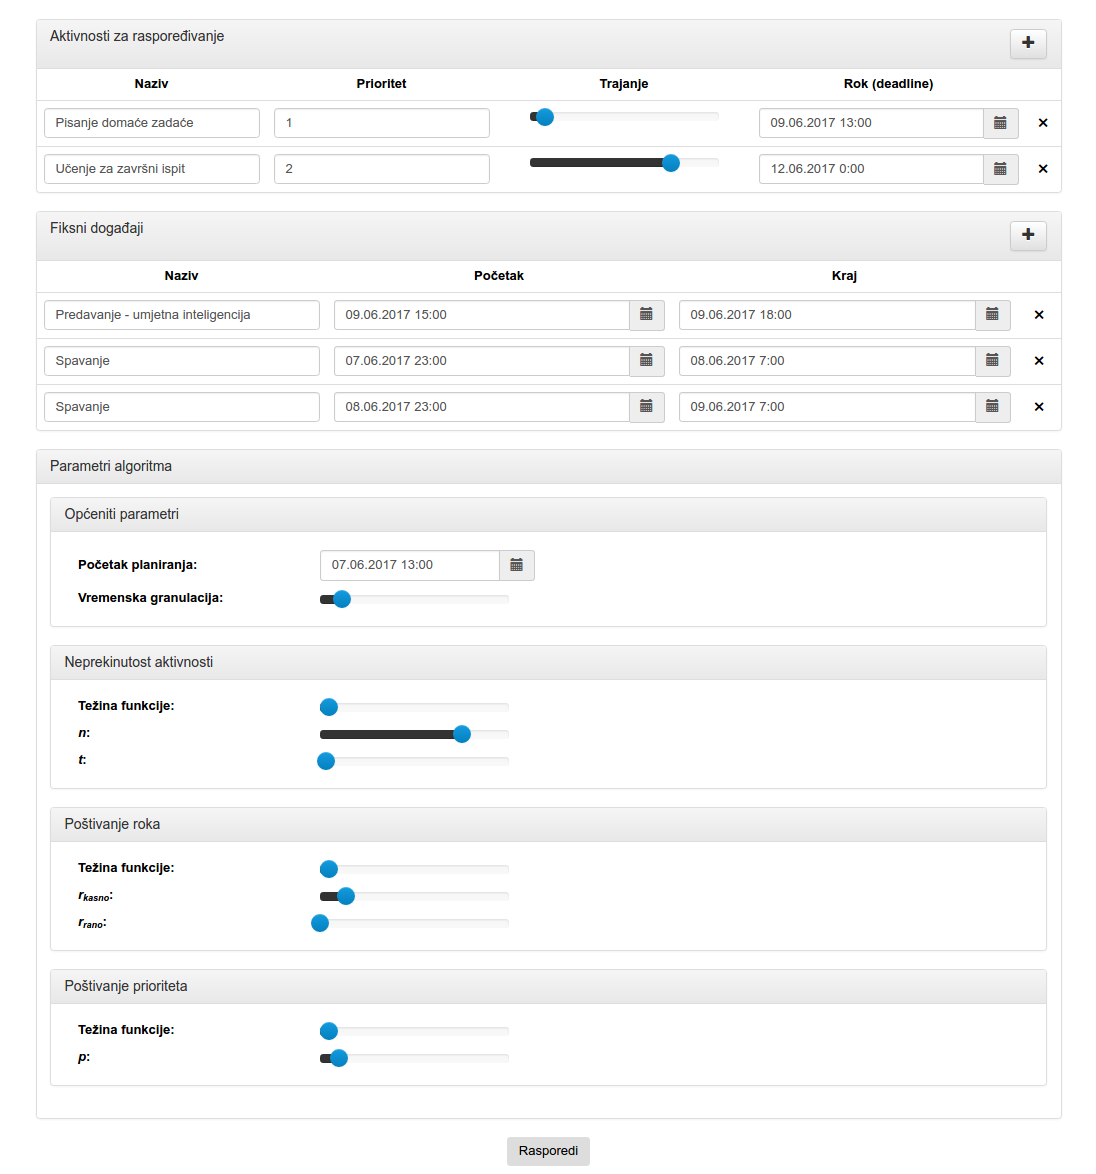
\includegraphics[width=\textwidth]{resources/graphics/screenshot-form.png}
\caption{Forma za unos ulaznih podataka}
\label{img:forma}
\end{figure}

\begin{figure}[]
\centering
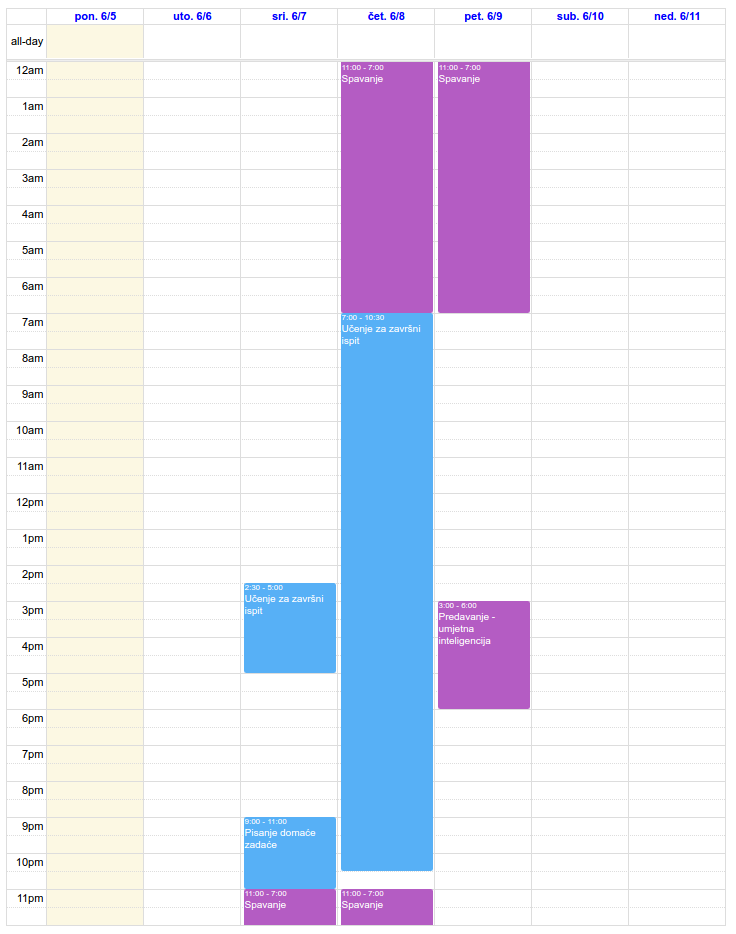
\includegraphics[width=\textwidth]{resources/graphics/screenshot-raspored-1.png}
\caption{Tjedni prikaz rasporeda}
\label{img:weekly_calendar}
\end{figure}

\iffalse
\chapter{Primjeri rezultata}\label{primjeri}
TODO:
- nekoliko primjera rasporeda s istim zadacima i različitim parametrima
\fi

\chapter{Zaključak}
Priroda je oduvijek inspirirala čovjekove ideje, razmišljanja i postupke. Kroz 4 milijarde godina, prirodni procesi su na Zemlji razvili život od najjednostavnijih jednostaničnih organizama do sisavaca koji su sposobni komunicirati, donositi racionalne odluke te učiti iz svijeta oko sebe. Proučavanjem upravo tih evolucijskih procesa moguće je konstruirati metode -- \textit{algoritme evolucijskog računanja} -- koji se vrlo dobro mogu nositi s teškim problemima koje klasičnim pristupom računalno ne bismo mogli riješiti.

U ovom radu predstavili smo problem slaganja osobnog kalendara kao optimizacijski problem i vidjeli kako ga se može riješiti primjenom genetskog algoritma. Upoznali smo se s implementacijskim elementima potrebnim za realizaciju sustava koji automatizirano slaže osobni raspored, od modela i biblioteka trećih strana do samih ideja evaluacijskih funkcija koje su osnova za rješavanje optimizacijskih problema.

Upoznali smo se i s genetskim algoritmom kao jednim od algoritama evolucijskog računanja, koji se često koristi za rješavanje raznih varijanti problema raspoređivanja. Izrada osobnog rasporeda, razložena u ovom radu, samo je jedan od takvih problema koji dobro ilustrira generalni pristup ovakvim problemima.

\paragraph{}
Daljnji razvoj sustava može se podijeliti u dvije kategorije. S jedne strane, moguće je razviti naprednije web sučelje za upravljanje sustavom, budući da trenutno sučelje pruža tek minimalan skup kontrola i nikakvu mogućnost upravljanja rezultatima. Dodatno se može implementirati integracija s alatima poput \textit{Google Kalendara}\footnote{https://calendar.google.com} i to-do listama (npr. \textit{Google Keep}\footnote{https://keep.google.com}, \textit{Trello}\footnote{https://trello.com}, \dots). S druge strane, sam algoritam se može razvijati implementirajući nova pravila, promjenom postojećih te uvođenjem novih funkcionalnosti ili parametara.

\paragraph{}
K\^{o}d rješenja dostupan je na Github repozitoriju: https://github.com/the-JJ/zavrsni-rad .


\bibliography{literatura}
\bibliographystyle{fer}

\begin{sazetak}
Automatizirano planiranje i raspoređivanje aktivnosti spada u razred $\mathcal{NP}$-teških problema. U ovom radu se taj problem definira kao optimizacijski problem te se izlaže način njegovog rješavanja primjenom genetskog algoritma. Definiraju se evaluacijske funkcije te biraju prigodni operatori selekcije, križanja i mutacije. U sklopu rada razvija se sustav s web sučeljem koji za zadani ulazni skup ograničenja i aktivnosti koje je potrebno rasporediti stvara raspored koji sadrži zadane aktivnosti i zadovoljava zadana ograničenja.

\kljucnerijeci{raspoređivanje aktivnosti, automatizirano planiranje i raspoređivanje, optimizacijski problem, genetski algoritam, evolucijsko računanje, metaheuristika}
\end{sazetak}

% TODO: Navedite naslov na engleskom jeziku.
\engtitle{Web Application for Activity Schedule Management}
\begin{abstract}
Automated activity planning and scheduling belongs to the $\mathcal{NP}$-hard class of problems. This paper presents such problem as an optimisation problem and offers methods for solving it using genetic algorithms. Covered topics include defining evaluation functions and selection of genetic operators -- selection, recombination and mutation. A constrained system with web interface for automated planning and scheduling of a set of given personal activities is developed.

\keywords{Activity Scheduling, Automated Planning and Scheduling, Optimisation Problem, Genetic Algorithm, Evolutionary Computing, Metaheuristics}
\end{abstract}

\end{document}
